\section{What is Bureaucracy?\label{sec:define-bureaucracy}}

While you may know it when you see or experience bureaucracy, for this book definitions are useful. Throughout the book we'll refer back to these definitions as we build out the concepts needed to understand bureaucracy.

\index{bureaucracy!definition of}
\Gls{bureaucracy} involves creation and execution of \glspl{policy} for managing shared resources. Creating and carrying out policies usually involves multiple people, with each person having specialized roles. Task scalability (how many widgets), complexity (number of tasks per widget), or latency (time per widget) motivate members with distinct roles to form a hierarchical organization to facilitate coordination. The organization has control over the disbursement of resources relevant to the society the organization operates within, or the organization administers a policy within that society. Resources managed by the organization are either tangible (e.g., water, air, land) or expertise.  

Bureaucracy is not limited to government. Non-profit organizations, volunteer groups, commercial companies, and even small teams of people can invoke bureaucratic tendencies. The existence of bureaucracy is independent of an organization's purpose, and independent of whether money is involved. Carrying out someone else's subjectively defined policy will require you to make your own subjective decisions regarding execution and enforcement. 

\ \\

With bureaucracy defined, distinct roles can be identified.
\index{bureaucracy!roles}
A bureaucracy typically involves a policy creator, a policy enforcer, and the person upon whom policy is inflicted. In the context of government, the policy creator can be either a politician or a bureaucrat. 

An organization comprised of bureaucrats is a \gls{bureaucracy}. The main character within a bureaucracy is the \gls{bureaucrat} -- the person who is a member of an organization and is responsible for subjective implementation of policy for the organization. The person that a bureaucrat's decisions are inflicted on a \gls{subject}.  Depending on context, a subject may be a student (when the bureaucrat is a teacher) or a subject may be a citizen if the bureaucrat is a police officer or government official. Sometimes a bureaucrat's decisions are inflicted on other bureaucrats-as-subjects, such as when a Chief of Police creates guidelines for police in their district, or when a senior diplomat sets policy for embassy employees. 


A \gls{bureaucrat} is a person subjectively interpreting policies on behalf of an organization and has discretionary enforcement. The bureaucrat's purpose is to facilitate coordination of stakeholders by applying specialized knowledge. 

Let's break that down piece-by-piece. First, ``subjective interpretation'' means there is a person making a decision about how to do something. The subjectivity arises from different reasons one person might choose an option over a competing option.  A \gls{policy} is a set of actions in a given circumstance. An \gls{organization} is the collection of people for who the policy is made. Discretionary enforcement means the person is choosing how to apply the policy in the specific circumstances. Facilitating coordination means bureaucracy is about getting multiple people (or sometimes a person at different instances in time) to work together. The stakeholders are people who care about the application of the action in each circumstance.  That's still pretty dense, so the rest of the book is spent expanding the nuances and implications of this definition.

Bureaucracy is neither good nor bad. Bureaucracy is not tied to politics, nor is bureaucracy specific to an institution (corporations, governments, academia). The definition of bureaucracy used in this book is independent of government. Bureaucracy is not defined to be efficient; nor does it have to be inefficient. Bureaucracy is not restricted to paperwork, record keeping, quantification, or gathering metrics. Nothing in this definition involves paperwork or an office building. Definitions that limit the concept of bureaucracy to specific contexts result in a decreased ability to describe complex large-scale human organizations. 

Bureaucracy is about delegation of control, communication, decision making, coordination, and processes. Bureaucracy relies on negotiation. 

\begin{figure}
    \centering
    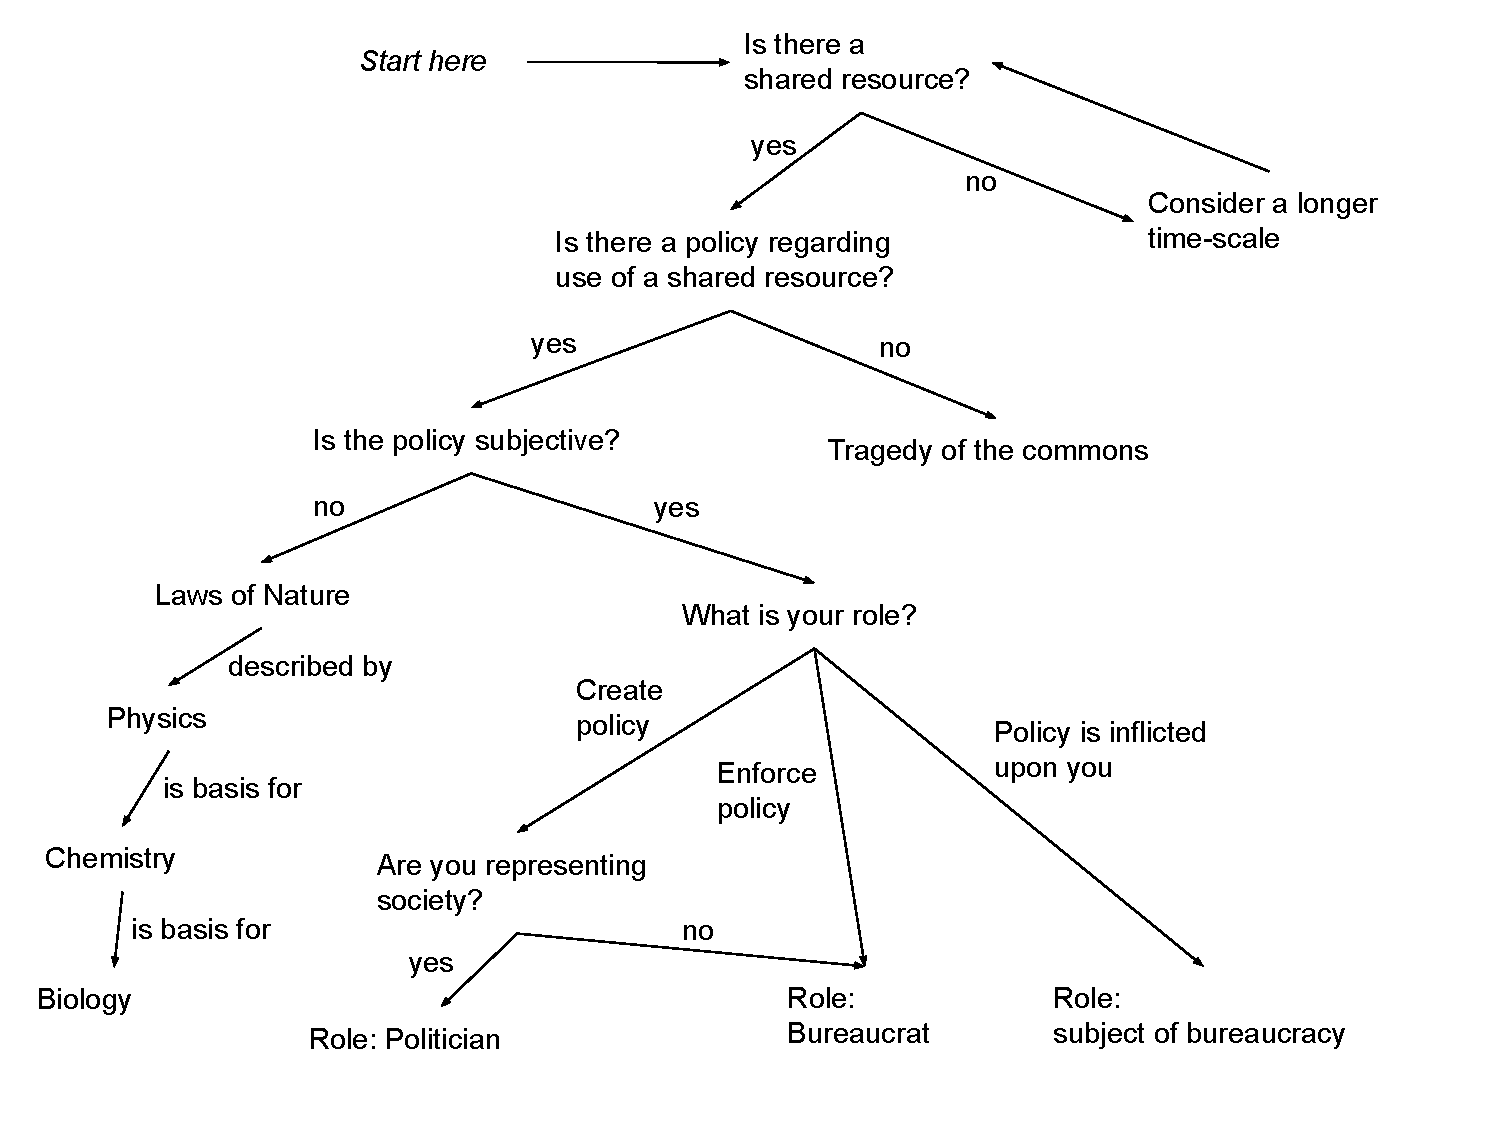
\includegraphics[width=1.05\textwidth]{images/am_I_a_bureaucrat.pdf}
    \caption{Decision tree for determining whether you qualify as a bureaucrat}
    \label{fig:am-I-a-bureaucrat}
\end{figure}

A critical aspect of bureaucracy is that everything is made up, specifically by other humans. The consequence is that everything is negotiable. You (in the role of either a subject or a bureaucrat) need to know both who to negotiate with and how to negotiate the desired changes. My claim that bureaucracy is made up is in contrast to actual rules -- the mathematical physics that describe nature. Everything in your environment is either naturally occurring macroscopic emergent phenomena (e.g., chemistry, biology) or humans making up labels and norms. Distinguishing the two is critical to knowing what you can change and what you have to operate within. 

Bureaucracy arises when there is no common, objectively quantifiable feedback mechanism for individual participants in the organization. This aspect is why governments, schools, and prisons are characterized as bureaucratic. The military doesn't rank soldiers by ``number of enemies killed'' and is bureaucratic. Even profit-driven commercial organizations are bureaucratic when the impacts of individual employees are not coupled to the metrics of profit. 

Profit-based feedback makes some roles in a business context slightly more predictable and understandable. Even in that situation there are trade-offs like externalization of costs and long-term profit versus short-term profit. 

The concept of bureaucracy is most visible for complex recurring situations involving many people and the control of a shared resource. The apparent friction of bureaucratic processes can be lower when there are only a few people involved (``I'm just talking to my collaborator" or ``I'm just buying groceries from a clerk at the store'' or ``I'm using a website for a government service''), but there is a continuous gradient to more obvious instances of bureaucracy. Bureaucratic tendencies are observable at the small scale; they typically get ignored or called something else.

Bureaucracy arises when management of a shared resource is necessary; that resource can be external to the organization or internal to the organization. Examples of external resources include mail delivery for \href{https://en.wikipedia.org/wiki/United_States_Postal_Service}{USPS}, public safety for \href{https://en.wikipedia.org/wiki/Federal_Bureau_of_Investigation}{FBI}, and the environment for \href{https://en.wikipedia.org/wiki/United_States_Environmental_Protection_Agency}{EPA}. The focus of this book is on internal resources. Resources internal to a bureaucratic organization include intangibles like attention, skill, expertise. Metrics like time, money, and staffing are proxy measures for the central intangible resources.



Bureaucracy is a system for distributed knowledge and distributed decision making. 
\index{bureaucracy!definition of}
That is in contrast to easier-to-understand concepts like centralized knowledge and centralized decision making. A government run by dictatorship is easy to conceptualize compared to democracies because there is a central character around which a narrative can be formed. Similarly, stories about the \href{https://en.wikipedia.org/wiki/Chief_executive_officer}{CEO} of a company are much easier than capturing the thousands of interactions conducted by the many employees of that company. The vast majority of the work an organization does is coordinated and carried out by people other than the CEO. Linear story-telling with a small number of main characters does not map well to the complexities of bureaucracy. 


